\documentclass[titlepage]{article}

\usepackage{alltt}
\usepackage{ifthen}
\usepackage{fancybox}
\usepackage{fancyvrb}
\usepackage{fancyhdr}
\usepackage[x11names]{xcolor}                     %Additional colors
%\usepackage[margin=1.1in,left=1.7in,right=1.7in]{geometry}
\usepackage[margin=1.1in]{geometry}
\usepackage{lastpage}
\usepackage{calc}
\usepackage{graphicx}  
\usepackage{hyperref}
\usepackage{tikz}
\usepackage{parskip}     % I rather this

%\hoffset = -0.5in
%\voffset = -0.5in
%\textheight = \textheight + 1in

\pagestyle{fancy}
\fancyhead[HL]{ENGR 108}
\fancyhead[HC]{Fall 2013}
\fancyhead[HR]{Computer Science / EECS}
\fancyfoot[FC]{\thepage{} of \pageref{LastPage}}

\newboolean{Sample}
\setboolean{Sample}{false}
\pagenumbering{arabic}

\shadowsize=1pt
\newcommand{\tickbox}{\raisebox{-2pt}{\shadowbox{\parbox{4pt}{~}}}}
\newcommand{\drawbox}[1]{\noindent\shadowbox{\parbox{\linewidth-8pt}{\vspace{#1em}~}}\newline}
\newcommand{\truefalse}{\dotfill\parbox{50pt}{~\tickbox{}~~~~~\tickbox{}~}}
% \raisebox{-1pt}{True:}\tickbox{}~~\raisebox{-1pt}{False:}\tickbox{}
\newcommand{\blankline}[1][100pt]{\underline{\parbox{#1}{~}}}
\def\sx{1.6in}


\begin{document}

\section*{Lab Summary}
\noindent
Your mission is to help us escape from Crater Lake.
\begin{itemize}
\item The game can be found at URL \url{http://www.ittc.ku.edu/~andygill/engr108/}
\end{itemize}
This puzzle is based on a classical math puzzle, attributed to Martin Gardner.
A recent writeup can be found at the following link. ({\bf not needed to complete lab.\/})
\begin{itemize}
\item \url{http://www.datagenetics.com/blog/october12013/}
\end{itemize}

\section*{Team Members}

\noindent(write the members of your team in this box).\\
\drawbox{9}

\section*{Controlling the raft}

To control the raft, simply \underline{assign the variable {\tt dir} with the radian
direction} you need to go. Because the raft has GPS, the directions are absolute;
$\pi/2$ will always make the raft go North.

Here is a summary of radians.

\begin{center}
  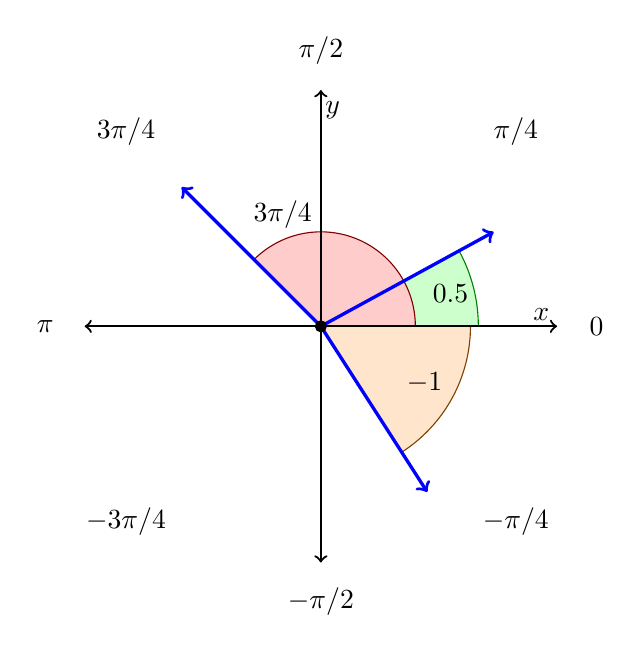
\begin{tikzpicture}
    % back arc 
    \filldraw[fill=green!20!white, draw=green!50!black]
      (0,0) -- (2,0) arc (0:0.5 r:2) -- cycle;
    \filldraw[fill=orange!20!white, draw=orange!50!black]
      (0,0) -- (1.9,0) arc (0:-1 r:1.9) -- cycle;
    \filldraw[fill=red!20!white, draw=red!50!black]
      (0,0) -- (1.2,0) arc (0:3 * pi / 4 r:1.2) -- cycle;
    %Main rays
    \foreach \a in {0, 90,...,359}
      \draw[->, thick] (0, 0) -- (\a:3);
    % Example
      \draw[blue, ->, very thick] (0, 0) -- (0.5 r:2.5);
      \draw (0.25 r: 1.7) node {$0.5$};

      \draw[blue, ->, very thick] (0, 0) -- (-1 r:2.5);
      \draw (-0.5 r: 1.5) node {$-1$};

      \draw[blue, ->, very thick] (0, 0) -- (3 * pi / 4 r:2.5);
      \draw (1.9 r: 1.5) node {$3\pi/4$};

    %Angle labels  
    \draw (0 r: 3.5) node {$0$};

    \draw (pi / 4 r: 3.5) node {$\pi/4$};
    \draw (pi / 2 r: 3.5) node {$\pi/2$};
    \draw (3 * pi / 4 r: 3.5) node {$3\pi/4$};

    \draw (pi r: 3.5) node {$\pi$};

    \draw (-pi / 4 r: 3.5) node {$-\pi/4$};
    \draw (-pi / 2 r: 3.5) node {$-\pi/2$};
    \draw (-3 * pi / 4 r: 3.5) node {$-3\pi/4$};

    % labels

    \draw (2.8,0.15) node {$x$};
    \draw (0.15,2.75) node {$y$};
    %Central point
    \draw[fill=black] (0,0) circle(0.7mm);

  \end{tikzpicture}
\end{center}

\newpage
\section{Programming the raft}

Goto \url{http://www.ittc.ku.edu/~andygill/engr108/}

Your screen should look something like:
\begin{center}
\framebox{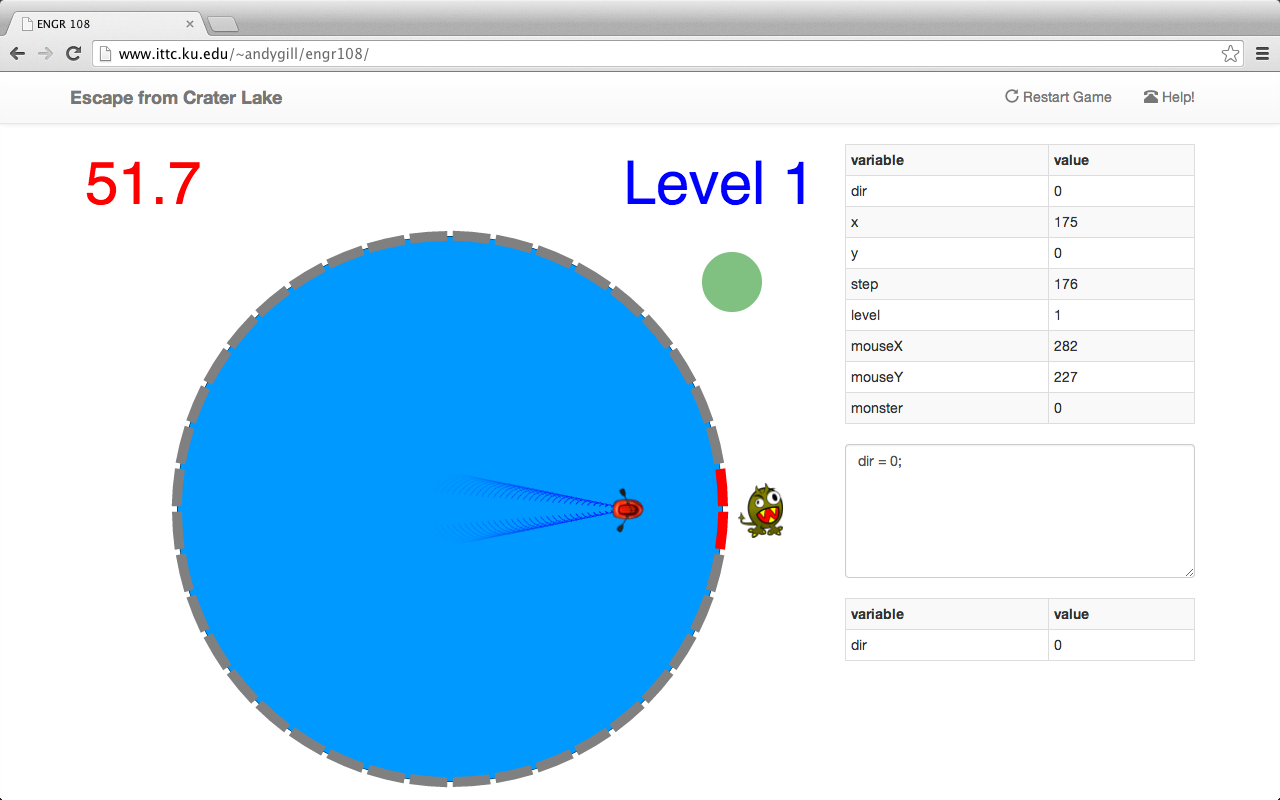
\includegraphics[trim = 25mm 0mm 25mm 28mm, clip,width=\textwidth - 2pt]{game.png}}
\end{center}

\begin{itemize}
\item The top is a navigation bar.
\begin{itemize}
\item You can restart the game. (Your program stays the same.)
\item You can bring up help.
\end{itemize}
\item The left hand side is Crater Lake.
\begin{itemize}
\item The raft is red.
\item The monster is running round the lake.
\item There is a green dot below the mouse.
\end{itemize}
\item The right hand side is the programming interface.
\begin{itemize}
\item You have a list of variables you can use.
\item You have an edit window where you write your code.
\item You have a list of variables after your program runs.
\item Your program runs continuously; click restart at the top right to restart.
\end{itemize} 
\end{itemize}

Good luck!

\newpage
\section{Sending the raft in one direction}

The first problem is to select a good first direction.

~\\
\noindent
Write and test the program to make the raft go {\bf West}.

\drawbox{4}

\noindent
Which of these initial directions are successful in escaping from the {\bf first} monster?

\parbox{10pt}{~}\ ~~~ \hfill\parbox{50pt}{Yes\hfill{}No~~~}
\begin{itemize}
\item when dir is $2$            \truefalse{}
\item when dir is $\pi$          \truefalse{}
\item when dir is $3.14$         \truefalse{}
\item when dir is $\pi - 0.1$    \truefalse{}
\end{itemize}

~\\
\noindent
Why is setting a single direction once a poor strategy overall?

\drawbox{7}

\section*{Programming Hints}

Assignments have the form 
{\Large\begin{quotation}
variable \verb|=| expression~;
\end{quotation}}

\begin{itemize}
\item {\em Variables\/} are upper or lower case, or mixtures of both. Upper case is (by convention)
used for variables that should never be changed.
\item {\em Expressions\/} are mathematical formula, including mathematical operations
(\verb|+|, \verb|-|, \verb|*|, \verb|/|), variables names, and parenthesis.
\end{itemize}

\subsection*{Useful Variables}

Here are some variables you may find useful for this exercise.

\begin{center}
\noindent
\begin{tabular}{rl}
\hline
{\bf Variable Name}     & Meaning\\
\hline
\verb|dir|              & direction the raft is traveling, in radians.\\
\verb|PI|               & $\pi$, or approximately 3.14159.\\
\hline
\end{tabular}        
\end{center}

\newpage

\section{Follow the mouse}

In this question, you need to add specific assignments that will make the raft follow the mouse.

The mouse coordinates can be found in the variables, \verb|mouseX| and \verb|mouseY|,
and the raft coordinates can be found in \verb|x| and \verb|y|.

\begin{center}
  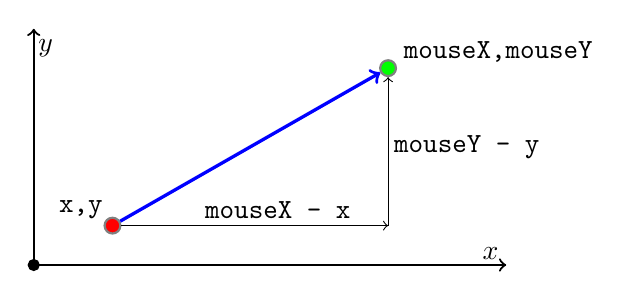
\begin{tikzpicture}
    %Main rays
    \draw[->, thick] (-3, 0) -- (3,0);
    \draw[->, thick] (-3, 0) -- (-3,3);

    % labels
    \draw (2.8,0.15) node {$x$};
    \draw (-3 + 0.15,2.75) node {$y$};
    %Central point
    \draw[fill=black] (-3,0) circle(0.7mm);

    % other lines
    
    \tikzstyle{place}=[circle,draw=black!50,fill=red,thick,inner sep=0pt,minimum size=2mm]

    % boat
    \node (raft) at (-2,0.5) [place] {};
    \draw (-2.4,0.7) node {\mbox{\tt x,y}};

    \node (mouse) at (1.5,2.5) [place,fill=green] {};
    \draw (2.9,2.7) node {\mbox{\tt mouseX,mouseY}};

    \draw[blue, ->, very thick] (raft) -- (mouse);

    \draw[black, ->] (raft) -- (1.5,0.5);
    \draw[black, ->] (1.5,0.5) -- (mouse);
    \draw (0.1,0.7) node {\mbox{\tt mouseX - x}};
    \draw (2.5,1.5) node {\mbox{\tt mouseY - y}};

  \end{tikzpicture}
\end{center}

There is a built-in function, \verb|atan2|, which, given a $y$ and $x$ coordinate,
computes the correct radian for you. For example, \verb|atan2|$(2,1)$ returns $1.107$,
and \verb|atan2|$(-1,3)$ returns $-0.322$. Note that the $y$ is the {\em first\/} argument.

First, make the raft go Southwest using \verb|atan2|. Remember, you need to assign \verb|dir|.

\drawbox{4}

Next, assign the variables \verb|dirX| and \verb|dirY|, which indicates the direction
that would head towards the mouse (the green circular blob), and use the
variables \verb|dirX| and \verb|dirY| as arguments to \verb|atan2|. 
If this is successful, your raft will now follow the green blob, which is beneath
the mouse.

\drawbox{10}

\subsection*{Useful Variables}

Here are some additional variables you may find useful for this exercise.

\begin{center}
\noindent
\begin{tabular}{rl}
\hline
{\bf Variable Name}     & Meaning\\
\hline
\verb|x|                & $x$-value of the coordinates of the raft.\\
\verb|y|                & $y$-value of the coordinates of the raft.\\
\verb|mouseX|           & $x$-value of the coordinates of the mouse / green blob.\\
\verb|mouseY|           & $y$-value of the coordinates of the mouse / green blob.\\
\hline
\end{tabular}        
\end{center}

\newpage

\section{The Great Escape}

In this exercise, you are to program an escape from Crater Lake.
See if your program can reach {\bf Level 4}, or higher.
%
Typically, you set the direction on the {\em first\/} step.
\begin{verbatim}
if (step == 1) {
  dir = PI;
}  
\end{verbatim}

Then, in future steps, you choose a step to re-direct the raft, giving:
\begin{verbatim}
if (step == 1) {
  dir = PI;
}  
if (step == 100) {
  dir = 0;
}
\end{verbatim}
You can do this as often as you need, and can change any of the constants.
Remember, to check equality
you should use \verb|==|. You
can also use the standard operators (\verb$<$, \verb$<=$, \verb$>$, \verb$>=$). 
The functions \verb|sin|, \verb|cos|, \verb|atan2|, and \verb|sqrt| are also available for use.
You are free to program as you see fit, computing the best value
for \verb|dir| each time your program is run.

\drawbox{25}

\subsection*{Useful Variables}

There are a number of additional variables you can use to attempt to escape.

\begin{center}
\noindent
\begin{tabular}{rl}
\hline
{\bf Variable Name}     & Meaning\\
\hline
\verb|step|             & is how many steps the level has taken, starting at 1\\
\verb|level|            & is the level number.\\
\verb|monster|          & is the location of the monster, in radians.\\
\hline
\end{tabular}        
\end{center}




\end{document}
